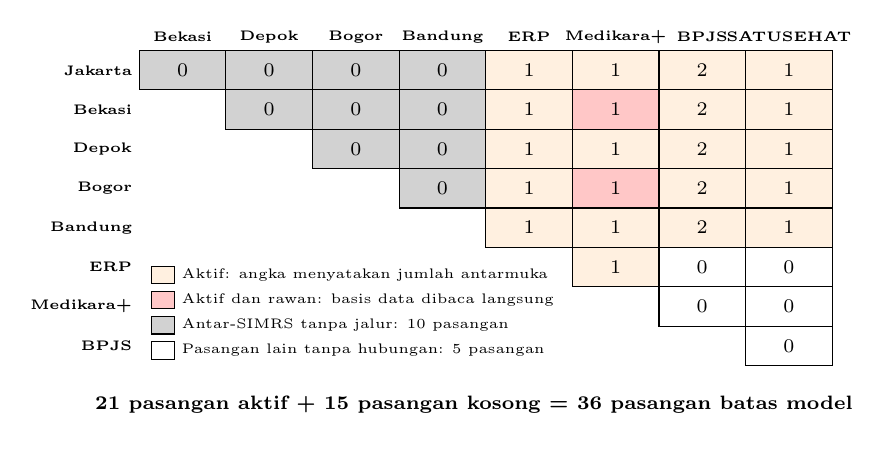
\begin{tikzpicture}[font=\scriptsize,
  sel/.style={draw, minimum width=1.1cm, minimum height=0.5cm, inner sep=0pt},
  aktif/.style={sel, fill=orange!12},
  rawan/.style={sel, fill=red!22},
  hampa/.style={sel, fill=gray!35},
  nol/.style={sel, fill=white},
  kepala/.style={font=\tiny\bfseries, inner sep=1pt},
  tanda/.style={draw, minimum width=0.3cm, minimum height=0.22cm, inner sep=0pt},
  ket/.style={font=\tiny, anchor=west, inner sep=1pt}]
  \foreach \kolom/\nama in {2/Bekasi, 3/Depok, 4/Bogor, 5/Bandung, 6/ERP,
      7/Medikara+, 8/BPJS, 9/SATUSEHAT} {
    \node[kepala] at (\kolom*1.1,0.42) {\nama};
  }
  \foreach \baris/\nama in {1/Jakarta, 2/Bekasi, 3/Depok, 4/Bogor, 5/Bandung,
      6/ERP, 7/Medikara+, 8/BPJS} {
    \node[kepala, anchor=east] at (1.6,-\baris*0.5+0.5) {\nama};
  }
  \foreach \baris/\kolom in {1/2, 1/3, 1/4, 1/5, 2/3, 2/4, 2/5, 3/4, 3/5, 4/5} {
    \node[hampa] at (\kolom*1.1,-\baris*0.5+0.5) {0};
  }
  \foreach \baris in {1,...,5} {
    \node[aktif] at (6*1.1,-\baris*0.5+0.5) {1};
    \node[aktif] at (8*1.1,-\baris*0.5+0.5) {2};
    \node[aktif] at (9*1.1,-\baris*0.5+0.5) {1};
  }
  \foreach \baris in {1,3,5} {
    \node[aktif] at (7*1.1,-\baris*0.5+0.5) {1};
  }
  \foreach \baris in {2,4} {
    \node[rawan] at (7*1.1,-\baris*0.5+0.5) {1};
  }
  \node[aktif] at (7*1.1,-6*0.5+0.5) {1};
  \foreach \baris/\kolom in {6/8, 6/9, 7/8, 7/9, 8/9} {
    \node[nol] at (\kolom*1.1,-\baris*0.5+0.5) {0};
  }
  \node[tanda, fill=orange!12] at (1.95,-2.6) {};
  \node[ket] at (2.15,-2.6) {Aktif: angka menyatakan jumlah antarmuka};
  \node[tanda, fill=red!22] at (1.95,-2.92) {};
  \node[ket] at (2.15,-2.92) {Aktif dan rawan: basis data dibaca langsung};
  \node[tanda, fill=gray!35] at (1.95,-3.24) {};
  \node[ket] at (2.15,-3.24) {Antar-SIMRS tanpa jalur: 10 pasangan};
  \node[tanda, fill=white] at (1.95,-3.56) {};
  \node[ket] at (2.15,-3.56) {Pasangan lain tanpa hubungan: 5 pasangan};
  \node[font=\scriptsize\bfseries] at (5.9,-4.25)
    {21 pasangan aktif + 15 pasangan kosong = 36 pasangan batas model};
\end{tikzpicture}
